\documentclass[twoside]{book}

% Packages required by doxygen
\usepackage{fixltx2e}
\usepackage{calc}
\usepackage{doxygen}
\usepackage[export]{adjustbox} % also loads graphicx
\usepackage{graphicx}
\usepackage[utf8]{inputenc}
\usepackage{makeidx}
\usepackage{multicol}
\usepackage{multirow}
\PassOptionsToPackage{warn}{textcomp}
\usepackage{textcomp}
\usepackage[nointegrals]{wasysym}
\usepackage[table]{xcolor}

% Font selection
\usepackage[T1]{fontenc}
\usepackage[scaled=.90]{helvet}
\usepackage{courier}
\usepackage{amssymb}
\usepackage{sectsty}
\renewcommand{\familydefault}{\sfdefault}
\allsectionsfont{%
  \fontseries{bc}\selectfont%
  \color{darkgray}%
}
\renewcommand{\DoxyLabelFont}{%
  \fontseries{bc}\selectfont%
  \color{darkgray}%
}
\newcommand{\+}{\discretionary{\mbox{\scriptsize$\hookleftarrow$}}{}{}}

% Page & text layout
\usepackage{geometry}
\geometry{%
  a4paper,%
  top=2.5cm,%
  bottom=2.5cm,%
  left=2.5cm,%
  right=2.5cm%
}
\tolerance=750
\hfuzz=15pt
\hbadness=750
\setlength{\emergencystretch}{15pt}
\setlength{\parindent}{0cm}
\setlength{\parskip}{3ex plus 2ex minus 2ex}
\makeatletter
\renewcommand{\paragraph}{%
  \@startsection{paragraph}{4}{0ex}{-1.0ex}{1.0ex}{%
    \normalfont\normalsize\bfseries\SS@parafont%
  }%
}
\renewcommand{\subparagraph}{%
  \@startsection{subparagraph}{5}{0ex}{-1.0ex}{1.0ex}{%
    \normalfont\normalsize\bfseries\SS@subparafont%
  }%
}
\makeatother

% Headers & footers
\usepackage{fancyhdr}
\pagestyle{fancyplain}
\fancyhead[LE]{\fancyplain{}{\bfseries\thepage}}
\fancyhead[CE]{\fancyplain{}{}}
\fancyhead[RE]{\fancyplain{}{\bfseries\leftmark}}
\fancyhead[LO]{\fancyplain{}{\bfseries\rightmark}}
\fancyhead[CO]{\fancyplain{}{}}
\fancyhead[RO]{\fancyplain{}{\bfseries\thepage}}
\fancyfoot[LE]{\fancyplain{}{}}
\fancyfoot[CE]{\fancyplain{}{}}
\fancyfoot[RE]{\fancyplain{}{\bfseries\scriptsize Generated by Doxygen }}
\fancyfoot[LO]{\fancyplain{}{\bfseries\scriptsize Generated by Doxygen }}
\fancyfoot[CO]{\fancyplain{}{}}
\fancyfoot[RO]{\fancyplain{}{}}
\renewcommand{\footrulewidth}{0.4pt}
\renewcommand{\chaptermark}[1]{%
  \markboth{#1}{}%
}
\renewcommand{\sectionmark}[1]{%
  \markright{\thesection\ #1}%
}

% Indices & bibliography
\usepackage{natbib}
\usepackage[titles]{tocloft}
\setcounter{tocdepth}{3}
\setcounter{secnumdepth}{5}
\makeindex

% Hyperlinks (required, but should be loaded last)
\usepackage{ifpdf}
\ifpdf
  \usepackage[pdftex,pagebackref=true]{hyperref}
\else
  \usepackage[ps2pdf,pagebackref=true]{hyperref}
\fi
\hypersetup{%
  colorlinks=true,%
  linkcolor=blue,%
  citecolor=blue,%
  unicode%
}

% Custom commands
\newcommand{\clearemptydoublepage}{%
  \newpage{\pagestyle{empty}\cleardoublepage}%
}

\usepackage{caption}
\captionsetup{labelsep=space,justification=centering,font={bf},singlelinecheck=off,skip=4pt,position=top}

%===== C O N T E N T S =====

\begin{document}

% Titlepage & ToC
\hypersetup{pageanchor=false,
             bookmarksnumbered=true,
             pdfencoding=unicode
            }
\pagenumbering{alph}
\begin{titlepage}
\vspace*{7cm}
\begin{center}%
{\Large solve-\/square }\\
\vspace*{1cm}
{\large Generated by Doxygen 1.8.13}\\
\end{center}
\end{titlepage}
\clearemptydoublepage
\pagenumbering{roman}
\tableofcontents
\clearemptydoublepage
\pagenumbering{arabic}
\hypersetup{pageanchor=true}

%--- Begin generated contents ---
\chapter{Main Page}
\label{index}\hypertarget{index}{}This program was create for solving the square equations\+: a$\ast$x$^\wedge$2 + b$\ast$x + c = 0. Thanks for using =)
\begin{DoxyItemize}
\item \hyperlink{main_8cpp}{main.\+cpp} 
\end{DoxyItemize}
\chapter{File Index}
\section{File List}
Here is a list of all documented files with brief descriptions\+:\begin{DoxyCompactList}
\item\contentsline{section}{\hyperlink{main_8cpp}{main.\+cpp} }{\pageref{main_8cpp}}{}
\end{DoxyCompactList}

\chapter{File Documentation}
\hypertarget{main_8cpp}{}\section{main.\+cpp File Reference}
\label{main_8cpp}\index{main.\+cpp@{main.\+cpp}}
{\ttfamily \#include $<$iostream$>$}\newline
{\ttfamily \#include $<$cmath$>$}\newline
{\ttfamily \#include $<$stdio.\+h$>$}\newline
{\ttfamily \#include $<$cassert$>$}\newline
{\ttfamily \#include $<$ctype.\+h$>$}\newline
Include dependency graph for main.\+cpp\+:\nopagebreak
\begin{figure}[H]
\begin{center}
\leavevmode
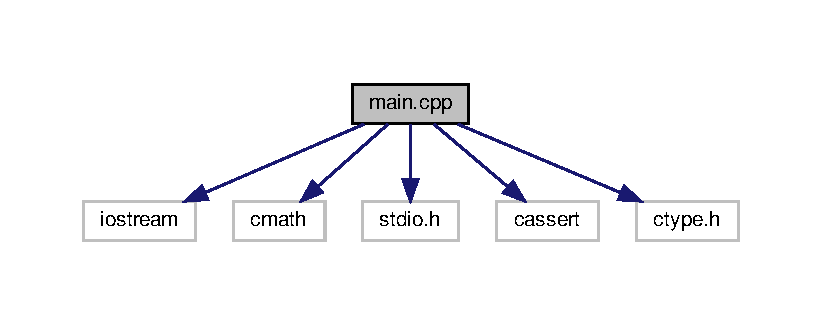
\includegraphics[width=350pt]{main_8cpp__incl}
\end{center}
\end{figure}
\subsection*{Macros}
\begin{DoxyCompactItemize}
\item 
\mbox{\Hypertarget{main_8cpp_a4520c2ed182d09cbb809b71c9226a77f}\label{main_8cpp_a4520c2ed182d09cbb809b71c9226a77f}} 
\#define {\bfseries M\+E\+OW}
\item 
\mbox{\Hypertarget{main_8cpp_ae1649fc947ca37a86917a08354f48d1a}\label{main_8cpp_ae1649fc947ca37a86917a08354f48d1a}} 
\#define {\bfseries P\+R\+I\+N\+TF}~printf
\end{DoxyCompactItemize}
\subsection*{Functions}
\begin{DoxyCompactItemize}
\item 
int \hyperlink{main_8cpp_ab2dd9b24e0e487efdd1cd1f40dd3a023}{Solve\+Square} (double a, double b, double c, double $\ast$x1, double $\ast$x2)
\item 
int \hyperlink{main_8cpp_aaabeeccf3691fb6a0e4b27370dc0ea93}{Linear} (double b, double c, double $\ast$x1)
\item 
int \hyperlink{main_8cpp_a9754b33474b4929519aac545e6661ed5}{Quadratic} (double a, double b, double c, double $\ast$x1, double $\ast$x2)
\item 
int \hyperlink{main_8cpp_ae66f6b31b5ad750f1fe042a706a4e3d4}{main} ()
\end{DoxyCompactItemize}
\subsection*{Variables}
\begin{DoxyCompactItemize}
\item 
\mbox{\Hypertarget{main_8cpp_a61fe66f8a8a77050d213dfe9f8df6232}\label{main_8cpp_a61fe66f8a8a77050d213dfe9f8df6232}} 
const int {\bfseries Inf\+Roots} = -\/1
\end{DoxyCompactItemize}


\subsection{Function Documentation}
\mbox{\Hypertarget{main_8cpp_aaabeeccf3691fb6a0e4b27370dc0ea93}\label{main_8cpp_aaabeeccf3691fb6a0e4b27370dc0ea93}} 
\index{main.\+cpp@{main.\+cpp}!Linear@{Linear}}
\index{Linear@{Linear}!main.\+cpp@{main.\+cpp}}
\subsubsection{\texorpdfstring{Linear()}{Linear()}}
{\footnotesize\ttfamily int Linear (\begin{DoxyParamCaption}\item[{double}]{b,  }\item[{double}]{c,  }\item[{double $\ast$}]{x1 }\end{DoxyParamCaption})}

Linear -\/ auxiliary function if a = 0 (b$\ast$x + c = 0) 
\begin{DoxyParams}[1]{Parameters}
\mbox{\tt in}  & {\em b} & -\/ coefficient. \\
\hline
\mbox{\tt in}  & {\em c} & -\/ coefficient. \\
\hline
\mbox{\tt out}  & {\em x1} & -\/ the root. \\
\hline
\end{DoxyParams}
\mbox{\Hypertarget{main_8cpp_ae66f6b31b5ad750f1fe042a706a4e3d4}\label{main_8cpp_ae66f6b31b5ad750f1fe042a706a4e3d4}} 
\index{main.\+cpp@{main.\+cpp}!main@{main}}
\index{main@{main}!main.\+cpp@{main.\+cpp}}
\subsubsection{\texorpdfstring{main()}{main()}}
{\footnotesize\ttfamily int main (\begin{DoxyParamCaption}{ }\end{DoxyParamCaption})}

In main function we have conditions because of number of roots can be different. In fact, Solve\+Square solves how many roots we have \mbox{\Hypertarget{main_8cpp_a9754b33474b4929519aac545e6661ed5}\label{main_8cpp_a9754b33474b4929519aac545e6661ed5}} 
\index{main.\+cpp@{main.\+cpp}!Quadratic@{Quadratic}}
\index{Quadratic@{Quadratic}!main.\+cpp@{main.\+cpp}}
\subsubsection{\texorpdfstring{Quadratic()}{Quadratic()}}
{\footnotesize\ttfamily int Quadratic (\begin{DoxyParamCaption}\item[{double}]{a,  }\item[{double}]{b,  }\item[{double}]{c,  }\item[{double $\ast$}]{x1,  }\item[{double $\ast$}]{x2 }\end{DoxyParamCaption})}

Quadratic -\/ auxiliary function if a != 0 (a$\ast$x$^\wedge$2 + b$\ast$x + c = 0) 
\begin{DoxyParams}[1]{Parameters}
\mbox{\tt in}  & {\em a} & -\/ coefficient. \\
\hline
\mbox{\tt in}  & {\em b} & -\/ coefficient. \\
\hline
\mbox{\tt in}  & {\em c} & -\/ coefficient. \\
\hline
\mbox{\tt out}  & {\em x1} & -\/ one of the root. \\
\hline
\mbox{\tt out}  & {\em x2} & -\/ one of the root. \\
\hline
\end{DoxyParams}
\mbox{\Hypertarget{main_8cpp_ab2dd9b24e0e487efdd1cd1f40dd3a023}\label{main_8cpp_ab2dd9b24e0e487efdd1cd1f40dd3a023}} 
\index{main.\+cpp@{main.\+cpp}!Solve\+Square@{Solve\+Square}}
\index{Solve\+Square@{Solve\+Square}!main.\+cpp@{main.\+cpp}}
\subsubsection{\texorpdfstring{Solve\+Square()}{SolveSquare()}}
{\footnotesize\ttfamily int Solve\+Square (\begin{DoxyParamCaption}\item[{double}]{a,  }\item[{double}]{b,  }\item[{double}]{c,  }\item[{double $\ast$}]{x1,  }\item[{double $\ast$}]{x2 }\end{DoxyParamCaption})}

Solve\+Square -\/ function for solving the equation 
\begin{DoxyParams}[1]{Parameters}
\mbox{\tt in}  & {\em a} & -\/ coefficient. \\
\hline
\mbox{\tt in}  & {\em b} & -\/ coefficient. \\
\hline
\mbox{\tt in}  & {\em c} & -\/ coefficient. \\
\hline
\mbox{\tt out}  & {\em x1} & -\/ one of the root. \\
\hline
\mbox{\tt out}  & {\em x2} & -\/ one of the root. \\
\hline
\end{DoxyParams}

%--- End generated contents ---

% Index
\backmatter
\newpage
\phantomsection
\clearemptydoublepage
\addcontentsline{toc}{chapter}{Index}
\printindex

\end{document}
